\documentclass[xcolor=x11names]{beamer}
\usepackage[utf8]{inputenc}
\usepackage{ragged2e}
\usepackage{setspace}
\usepackage{booktabs}
\usepackage{amsmath}
\usepackage{mathtools}
\usepackage{amsmath,graphicx,subcaption}
\usepackage[lastpage,user]{zref}
\usepackage{fancyhdr}
\usepackage{txfonts}
\usepackage{multirow}
\usepackage{dcolumn}
\usepackage{etaremune}
\usepackage[T1]{fontenc}
\usepackage{mathptmx}
\usepackage{tikz}
\usetikzlibrary{arrows.meta,shapes,decorations.markings,positioning}
\usepackage{mathrsfs}
\usepackage{pifont}

\newcommand{\uni}{\cup}
\newcommand{\sus}{\subseteq}
\newcommand{\sis}{\supseteq}
\newcommand{\ex}{\exists}
\newcommand{\ria}{\rightarrow}
\newcommand{\Ria}{\Rightarrow}
\newcommand{\lea}{\leftarrow}
\newcommand{\Lea}{\Leftarrow}
\newcommand{\s}{\quad}
\newcommand{\Real}{\mathbf{R}}
\newcommand{\N}{\mathbf{N}}
\newcommand{\all}{\forall}
\newcommand{\nt}{\mathbb}
\newcommand{\al}{\alpha}
\newcommand{\be}{\beta}
\newcommand{\ga}{\gamma}
\newcommand{\de}{\delta}
\newcommand{\ep}{\epsilon}
\newcommand{\va}{\varepsilon}
\newcommand{\ka}{\kappa}
\newcommand{\la}{\lambda}
\newcommand{\ro}{\rho}
\newcommand{\si}{\sigma}
\newcommand{\nue}{\upsilon}
\newcommand{\ph}{\phi}
\newcommand{\om}{\omega}
\newcommand{\Om}{\Omega}
\newcommand{\De}{\Delta}
\newcommand{\Si}{\Sigma}
\newcommand{\tri}{\triangle}
\newcommand{\ba}{\begin{array}}
\newcommand{\ea}{\end{array}}
\newcommand{\bc}{\begin{center}}
\newcommand{\ec}{\end{center}}
\newcommand{\beq}{\begin{equation}}
\newcommand{\eeq}{\end{equation}}
\newcommand{\bbm}{\begin{bmatrix}}
\newcommand{\ebm}{\end{bmatrix}}
\newcommand{\bpr}{\begin{proof}}
\newcommand{\epr}{\end{proof}}
\newcommand{\bit}{\begin{itemize}}
\newcommand{\eit}{\end{itemize}}
\newcommand{\abs}{{\big |}}
\newcommand{\Abs}{{\Big |}}
\newcommand{\hli}{ \hrulefill }
\newcommand{\lab}{\label}
\newcommand{\pref}{\pageref}
\newcommand{\eq}{equation }
\newcommand{\fig}{figure }
\newcommand{\bfig}{\begin{figure} }
\newcommand{\efig}{\end{figure} }
\newcommand{\sy}{system }
\newcommand{\ic}{initial conditions }
\newcommand{\evl}{eigenvalues }
\newcommand{\evc}{eigenvectors }
\newcommand{\fr}[2]{\frac{}{}}
\newcommand{\btal}{\begin{table}}
\newcommand{\etal}{\end{table}}
\newcommand{\btab}{\begin{tabular}}
\newcommand{\etab}{\end{tabular}}
\newcommand{\C}{\mathbb{C}}
\newcommand{\R}{\mathbb{R}}
\newcommand{\ele}{\text{e}}
\newcommand{\del}{\bigtriangledown}
\newcommand{\Ep}{\varepsilon}
\newcommand{\kte}{\ka T_\ele}
\newcommand{\pdd}[2]{\frac{\partial^2 #1}{\partial #2^2}}
\newcommand{\pd}[2]{\frac{\partial #1}{\partial #2}}
\newcommand{\bra}[1]{\langle #1 \rangle}
\newcommand{\mev}{\text{MeV}}
\newcommand{\he}[1]{\text{He}^{#1}}
\newcommand{\li}[1]{\text{Li}^{#1}}
\newcommand{\ds}{\text{d}}
\newcommand{\dder}[2]{\frac{\ds^2 #1}{\ds #2^2}}
\newcommand{\der}[2]{\frac{\ds #1}{\ds #2}}
\newcommand{\bigp}[1]{\left(#1\right)}
\newcommand{\cross}[1]{\del\times\vec{#1}}
\newcommand{\dig}[1]{\del\cdot\vec{#1}}
\newcommand{\bigs}[1]{\left[#1\right]}
\newcommand{\mynote}[1]{\textcolor{red}{#1}}
\newcommand{\myqn}[1]{\textcolor{blue}{#1}}
\newcommand{\er}{$\vec{E_r}$ }
% \usepackage[usenames,dvipsnames]{color}
\newcommand{\cmod}{C-Mod }
\newcommand{\ddd}{DIII-D }
\newcommand{\imode}{I-mode }
\newcommand{\lmode}{L-mode }
\newcommand{\hmode}{H-mode }

\let\tempone\itemize
\let\temptwo\enditemize
% \renewenvironment{itemize}{\tempone\addtolength{\itemsep}{-0.5\baselineskip}}{\temptwo}
\beamertemplatenavigationsymbolsempty

\definecolor{INLblue}{rgb}{0.0246913, 0.32921810, 0.646090534} 
\setbeamercolor{frametitle}{fg=INLblue}
\setbeamercolor{section in head/foot}{fg=INLblue}
\setbeamercolor{author in head/foot}{fg=INLblue}
\setbeamercolor{date in head/foot}{fg=INLblue}
\setbeamercolor{normal text}{fg=INLblue}

\setbeamertemplate{itemize item}{\color{INLblue}{\tiny\ding{108}}}
\setbeamertemplate{itemize subitem}{\color{INLblue}$-$}
\setbeamertemplate{itemize subsubitem}{\color{INLblue}{\tiny\ding{108}}}
\setbeamertemplate{itemize subsubsubitem}{\color{INLblue}$-$}

\makeatletter
\setbeamertemplate{frametitle}{
    \ifbeamercolorempty[bg]{frametitle}{}{\nointerlineskip}%
    \@tempdima=\textwidth%
    \advance\@tempdima by\beamer@leftmargin%
    \advance\@tempdima by\beamer@rightmargin%
    \vspace*{.4cm}
    \hspace*{.75cm}
    % \hspace*{-5cm}
    \begin{beamercolorbox}[sep=0.3cm,wd=\the\@tempdima]{frametitle}
        \usebeamerfont{frametitle}%
        \vbox{}\vskip-1ex%
        \if@tempswa\else\csname beamer@ftecenter\endcsname\fi%
        \strut\insertframetitle\strut\par%
        {%
            \ifx\insertframesubtitle\@empty%
            \else%
            {\usebeamerfont{framesubtitle}\usebeamercolor[fg]{framesubtitle}\insertframesubtitle\strut\par}%
            \fi
        }%
        \vskip-1ex%
        \if@tempswa\else\vskip-.3cm\fi% set inside beamercolorbox... evil here...
    \end{beamercolorbox}%
}
\makeatother

\usebackgroundtemplate%
{%
    
\includegraphics[width=\paperwidth,height=\paperheight, page=2]{Images/Presentation1.pdf}%
}

\begin{document}
% can only compile from the main.tex

% \input{Slide1}
%%%%%%%%%%%%%%%%%%$$$$$$$$$$$$$$$$$$$$$$$$%%%%%%%%%%%%%%%%%%$$$$$$$$$$$$$$$$$$$$$$$$%%%%%%%%%%%%%%%%%%$$$$$$$$$$$$$$$$$$
\usebackgroundtemplate{
\includegraphics[width=\paperwidth,page=1]{../Images/Presentation1.pdf}}%
%%%%%%%%%%%%%%%%%%$$$$$$$$$$$$$$$$$$$$$$$$%%%%%%%%%%%%%%%%%%$$$$$$$$$$$$$$$$$$$$$$$$%%%%%%%%%%%%%%%%%%$$$$$$$$$$$$$$$$$$

\begin{frame}{}
    \begin{columns}[c]
        \begin{column}{.2\textwidth}
            \vspace{-1.9in}
        % Hyperspectral anomaly detection model was adapted from a computer vision model.
        % The HSI compares data points similarity and the density of pixels that are considered similar.
        % The HSI has been adapted to take any type of data generated by a splunk query 
            \begin{table}[]
                \begin{tabular}{l}
                    \textcolor{white}{\tiny{\today}}\\[4pt]
                    \textbf{\textcolor{white}{\footnotesize Dempsey Rogers}}\\
                    \textcolor{white}{\footnotesize AI/ML Data Scientist}
                \end{tabular}
            \end{table}
            
        \end{column}
            \hfill
        \begin{column}{.8\textwidth}
           \vspace{.45in}
        \end{column}
    \end{columns}
    
    \vspace{-.2in}
    \hspace{-.2in}
        
    \begin{table}[]
        \begin{tabular}{l}
            \textbf{\LARGE{Hyperspectral Imaging (HSI)}}\\[4pt] 
            \textbf{\LARGE{Anomaly Detection}}\\[4pt]
        \end{tabular}
    \end{table}
\end{frame}

%%%%%%%%%%%%%%%%%%$$$$$$$$$$$$$$$$$$$$$$$$%%%%%%%%%%%%%%%%%%$$$$$$$$$$$$$$$$$$$$$$$$%%%%%%%%%%%%%%%%%%$$$$$$$$$$$$$$$$$$
\usebackgroundtemplate{
\includegraphics[width=\paperwidth,page=2]{../Images/Presentation1.pdf}}%
%%%%%%%%%%%%%%%%%%$$$$$$$$$$$$$$$$$$$$$$$$%%%%%%%%%%%%%%%%%%$$$$$$$$$$$$$$$$$$$$$$$$%%%%%%%%%%%%%%%%%%$$$$$$$$$$$$$$$$$$



\begin{frame}{What is the HSI Model?}
    The HSI model is a \textbf{statistical} approach to \textbf{anomaly} detection.  HSI does not learn weights through training for later use during inference. 

    \hfill
    
    The model was selected for its use of edge and vertex weighted \textbf{graphs} to obtain relations between data points at different topological and \textbf{temporal scales} by evolving the affinity matrix. 

    \hfill   
    
    HSI was adapted from the paper: \textit{Graph Evolution-Based Vertex Extraction for Hyperspectral Anomaly Detection by Xianchang Yang et al.}
    \hfill
\end{frame}




% \section{What Does HSI Do?}
% \begin{frame}{Model Pipeline}
% \begin{columns}
% \begin{column}{.45\linewidth}
% \begin{itemize}
%     \item Pre-processing
%     \begin{itemize}
%         \item TFIDF IP by quads
%         \item Select Modeling Components with PVA
%     \end{itemize}
    
%     \item Model
%     \begin{itemize}
%         \item \alert<2>{Edge} and \alert<3>{Vertex} Weight Generation
%         \item \alert<4>{Affinity} and \alert<4>{other Graphs} 
%         \item Graph Evolution
%         \item \alert<5>{Penalized Objective Function}
%     \end{itemize}
    
%     \item Inference
%     \begin{itemize}
%         \item Data Selection
%         \item Behavior Exclusion
%         \item Multifilter
%     \end{itemize}
% \end{itemize}
% \end{column}
% \begin{column}{.55\linewidth}\hfill\vfill
% \alert<2>{ $\gamma_i=\sum_{i\neq j}e^{-\left( d_{ij}/d_c\right)^2} \,:\,\vec{\gamma}\in \mathbb{R}^n $ }\\\hfill\vfill
% \alert<3>{$s_{ij}=e^{\left(- d_{ij}/d_c^2 \right)}\,:\, \vec{S}\in \mathbb{R}^{n,n}$}\\\hfill\vfill
% \alert<4>{$ d_{i=j}=\left(\sum_j^n s_{ij}\right)^{-\frac{1}{2}} , d_{i\neq j}=0\,:\, \vec{D}\in \mathbb{R}^{n,n}$\\\hfill\vfill
% $\vec{A}=\vec{\Gamma}\tilde{S}\vec{\Gamma} \,:\, \vec{A}\in \mathbb{R}^{n,n}$\\
% }\hfill\vfill
% \alert<5>{$ f\left(\vec{m}\right)=\frac{1}{2}\vec{m}^T\vec{A}^k\vec{m}+\left(\vec{\gamma}^T\vec{D}\right)^T\vec{m} $}\hfill\vfill
% \end{column}
% \end{columns}


% \end{frame}

% \begin{frame}{Model Pipeline}\vspace{-.25in}
% \begin{columns}
% \begin{column}{.45\linewidth}
% \begin{itemize}
%     \item Pre-processing
%     \begin{itemize}
%         \item TFIDF IP by quads
%         \item Select Modeling Components with PVA
%     \end{itemize}
    
%     \item Model
%     \begin{itemize}
%         \item Edge and Vertex Weight Generation
%         \item Affinity and other Graphs 
%         \item Graph Evolution
%         \item Penalized Objective Function
%     \end{itemize}
    
%     \item Inference
%     \begin{itemize}
%         \item Data Selection
%         \item Behavior Exclusion
%         \item Multifilter
%     \end{itemize}
% \end{itemize}
% \end{column}
% \begin{column}{.55\linewidth}\vspace{-.5in}\bc
% 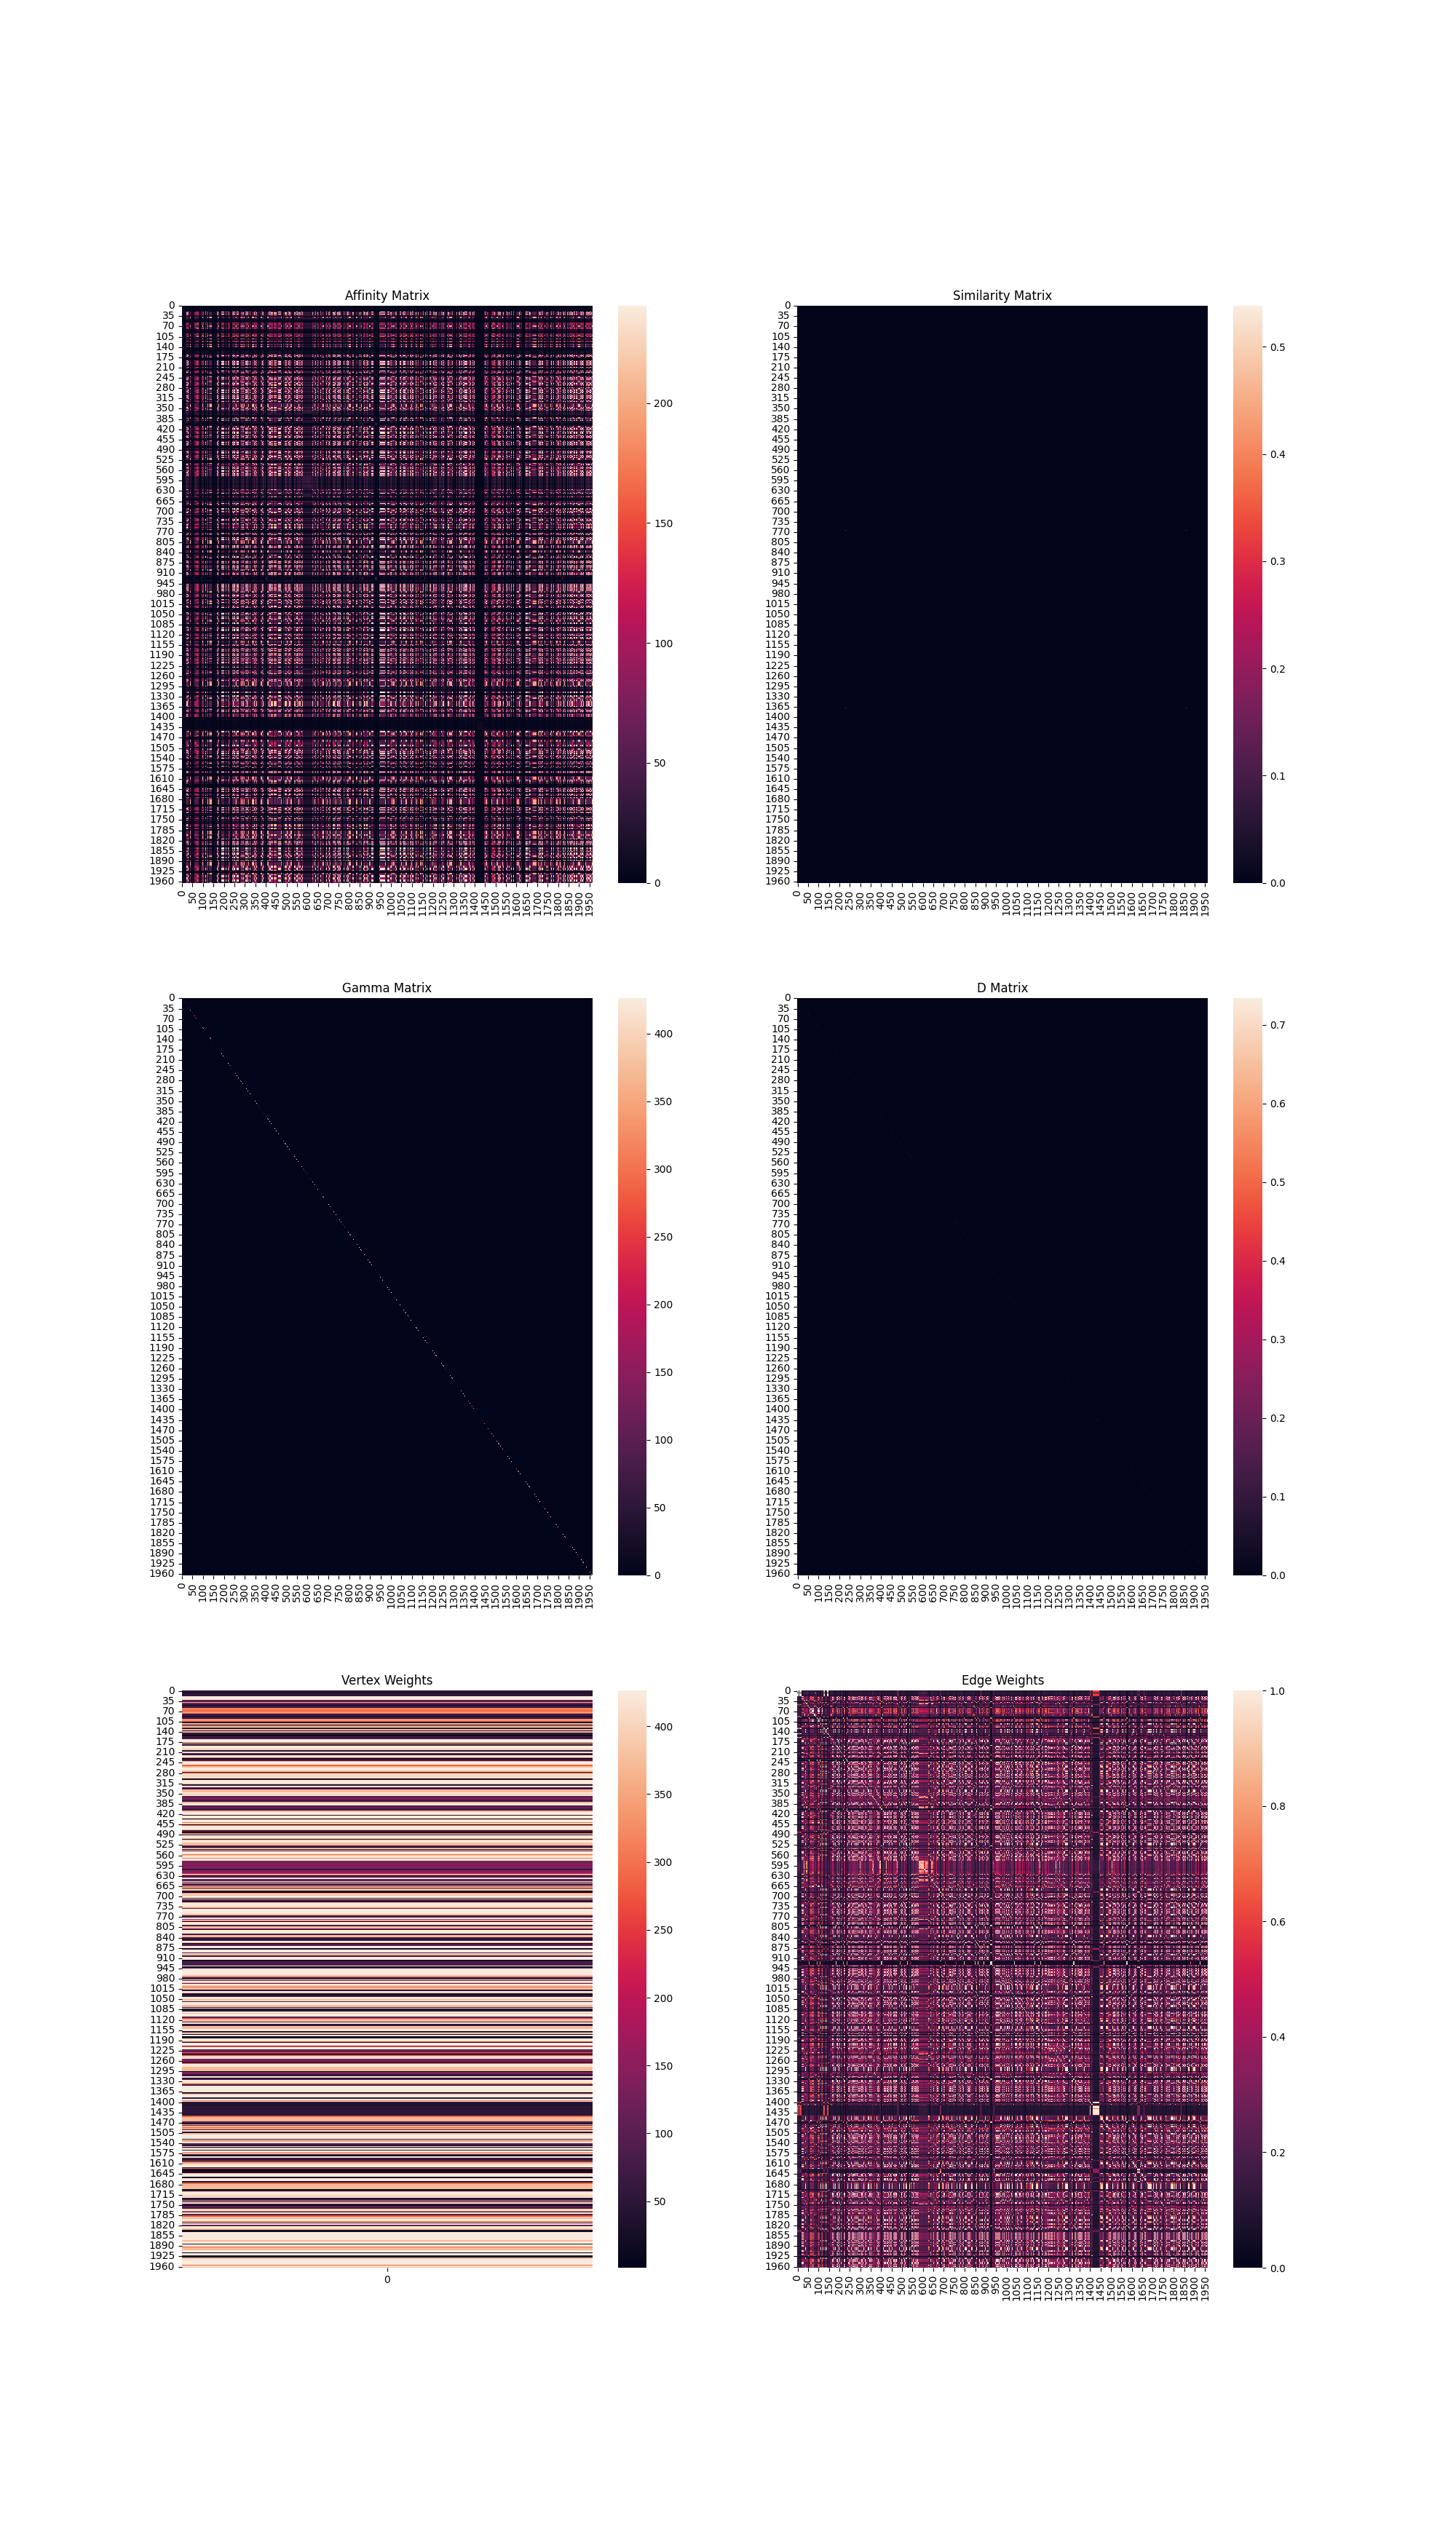
\includegraphics[clip=true, trim=2in 3.25in 2in 3.25in, height=.9\textheight, width=\textwidth ]{../Images/cb_protection_custom_model_weights.png}
% \ec\end{column}
% \end{columns}
% \end{frame}



\begin{frame}{Model Structure}
    The HSI model is broken down into two main components, \alert{weights generation} and {loss function minimization}. 

    \vfill
    
    \begin{columns}
        \begin{column}{.7\textwidth}
            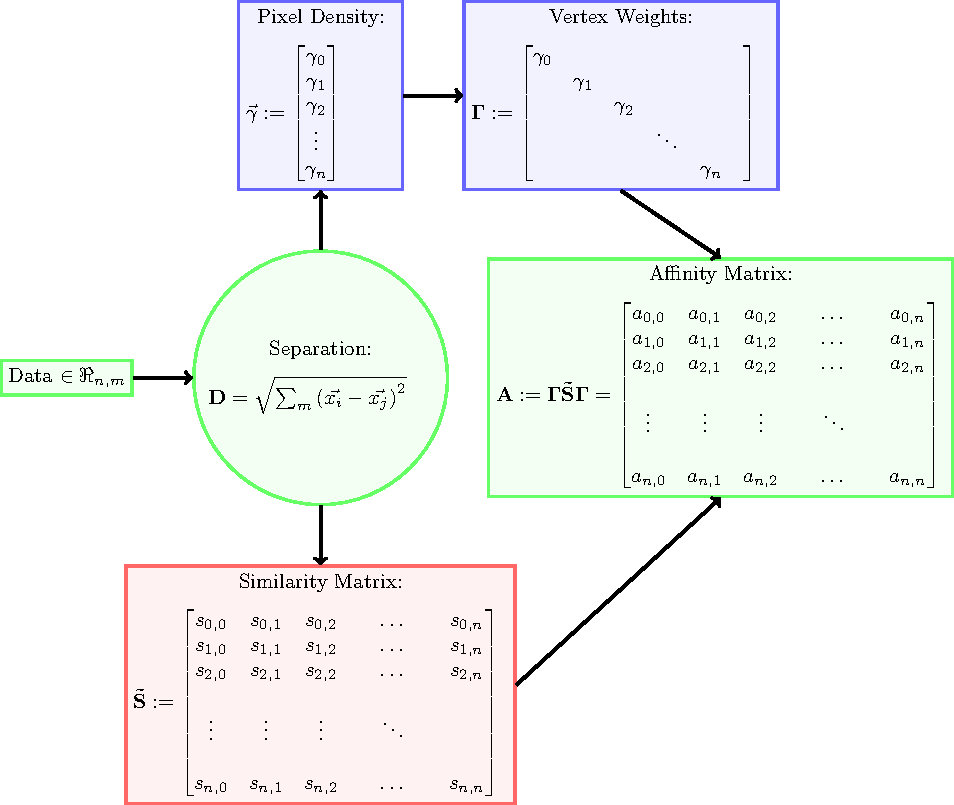
\includegraphics[width=\textwidth]{../Images/model_pipeline_tikz/Phase1_tikz/tikz.pdf}    
        \end{column}
        \begin{column}{.3\textwidth}
            \only<1>{
                \bc 
                    Density Calculations:\\
                    \vspace{.1in} 
                    $\gamma_i=\sum_{i\neq j}e^{-\left( d_{ij}/d_c\right)^2}$ 
                    \vspace{.1in}
                    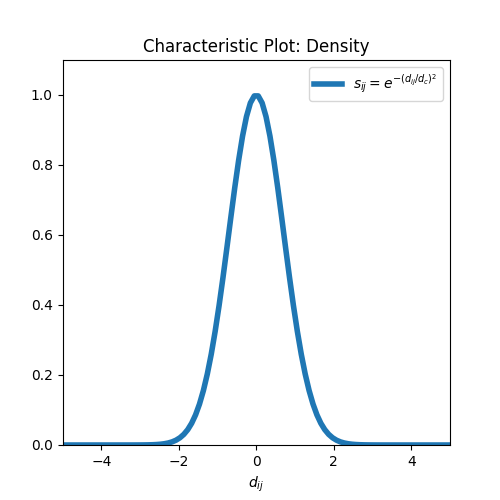
\includegraphics[width=1.2\textwidth]{../Images/density_plot.png}
                \ec
                }
            \only<2>{
                \bc 
                    Similarity Calculations:\\
                    \vspace{.1in} 
                    $s_{ij}=e^{\left(- d_{ij}/d_c^2 \right)}$   \vspace{.1in}
                    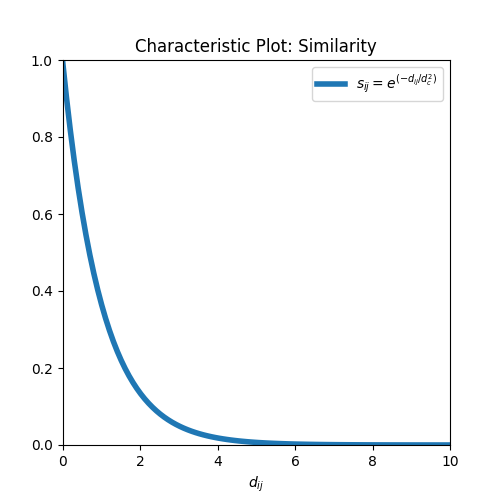
\includegraphics[width=1.2\textwidth]{../Images/similarity_plot.png}
                \ec}
        \end{column}
    \end{columns}
\end{frame}


\begin{frame}{Matrix Evolution \tiny{(aside)}}
    Adjacency matrices are used in graph theory to encode a graph's structure.
    \begin{columns}
        \begin{column}{.3\textwidth}
            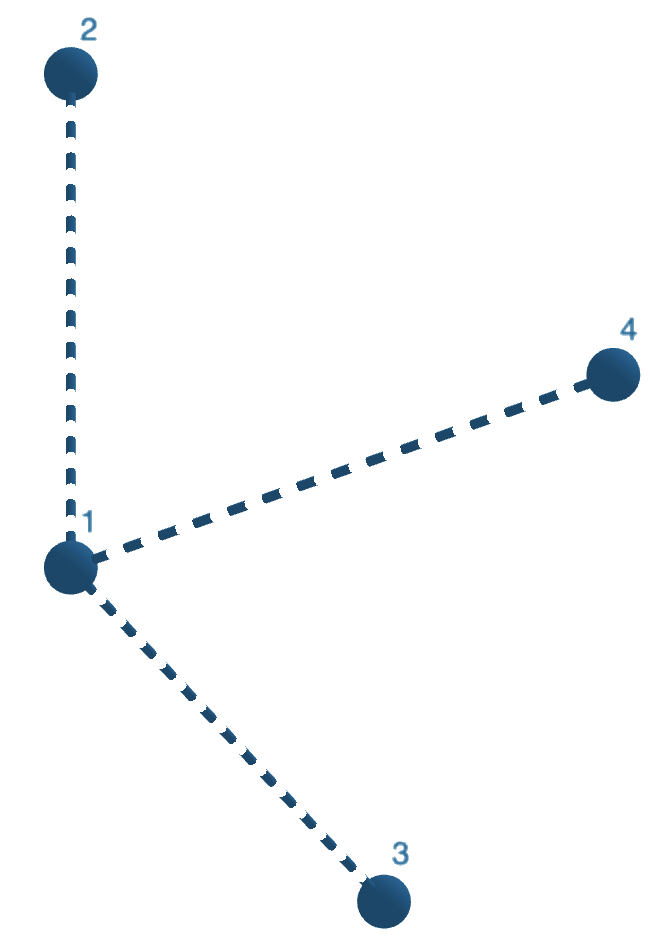
\includegraphics[width=.8\textwidth, clip=True, trim= 0in .05in 0in 0in]{../Images/my_graph.png}
        \end{column}        
        \begin{column}{.7\textwidth}
            Adjacency $\Ria$ Discrete
            \begin{itemize}
                \item Distance: Integer number of Hops
                \item Connectivity: Integer Number of Paths
            \end{itemize}
            Affinity $\Ria$ $\sim$Continuous 
            \begin{itemize}
                \item Distance: Function Space Measurement 
                \item Connectivity: Encoded in $\mathbf{A}$ and ${\vec{\gamma}}$
            \end{itemize}
        \end{column}
    \end{columns} 
    \bc
        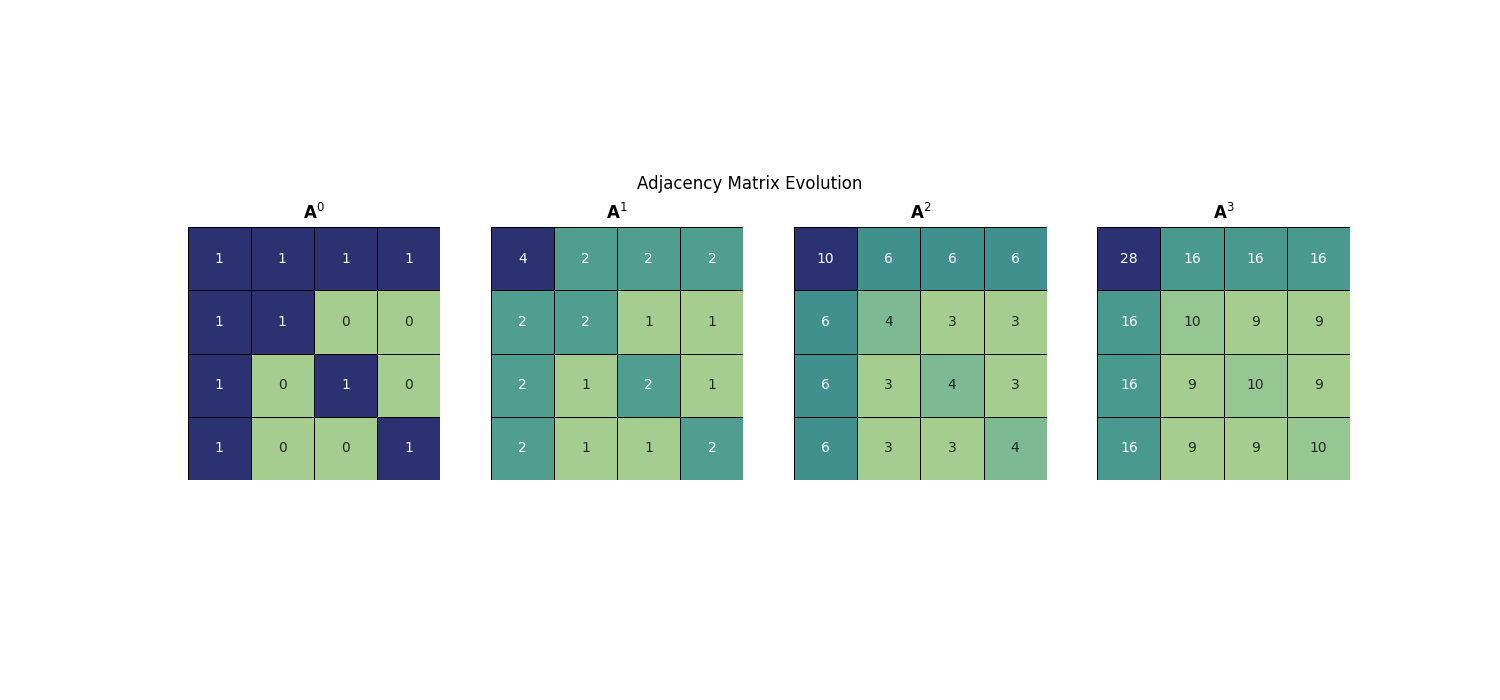
\includegraphics[width=.9\textwidth, clip=True, trim= 1.45in 2.15in 1.45in 1.75in]{../Images/matrix_evo.png}
    \ec    
\end{frame}

% \begin{frame}{Example Results and Reporting}
% Starting Splunk query refined with the analyst team:\\
% \begin{center}
%     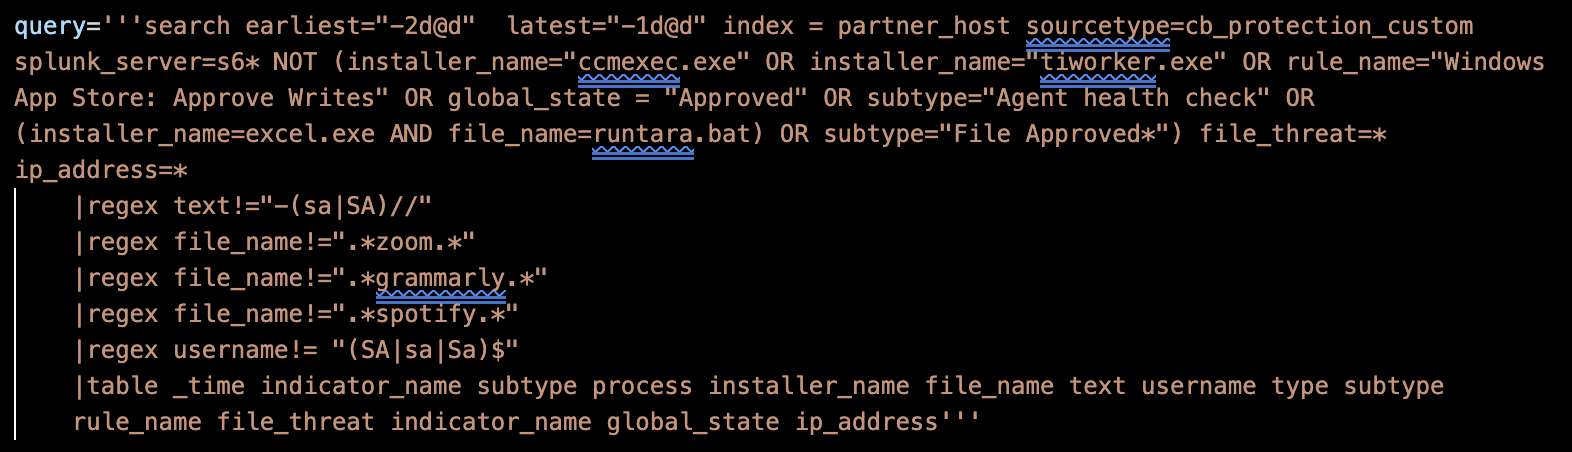
\includegraphics[width=\textwidth]{../Images/query.png}
% \end{center}

% \end{frame}

% \begin{frame}{Example Results and Reporting}
% HSI log for this query:\\
% \begin{center}
%     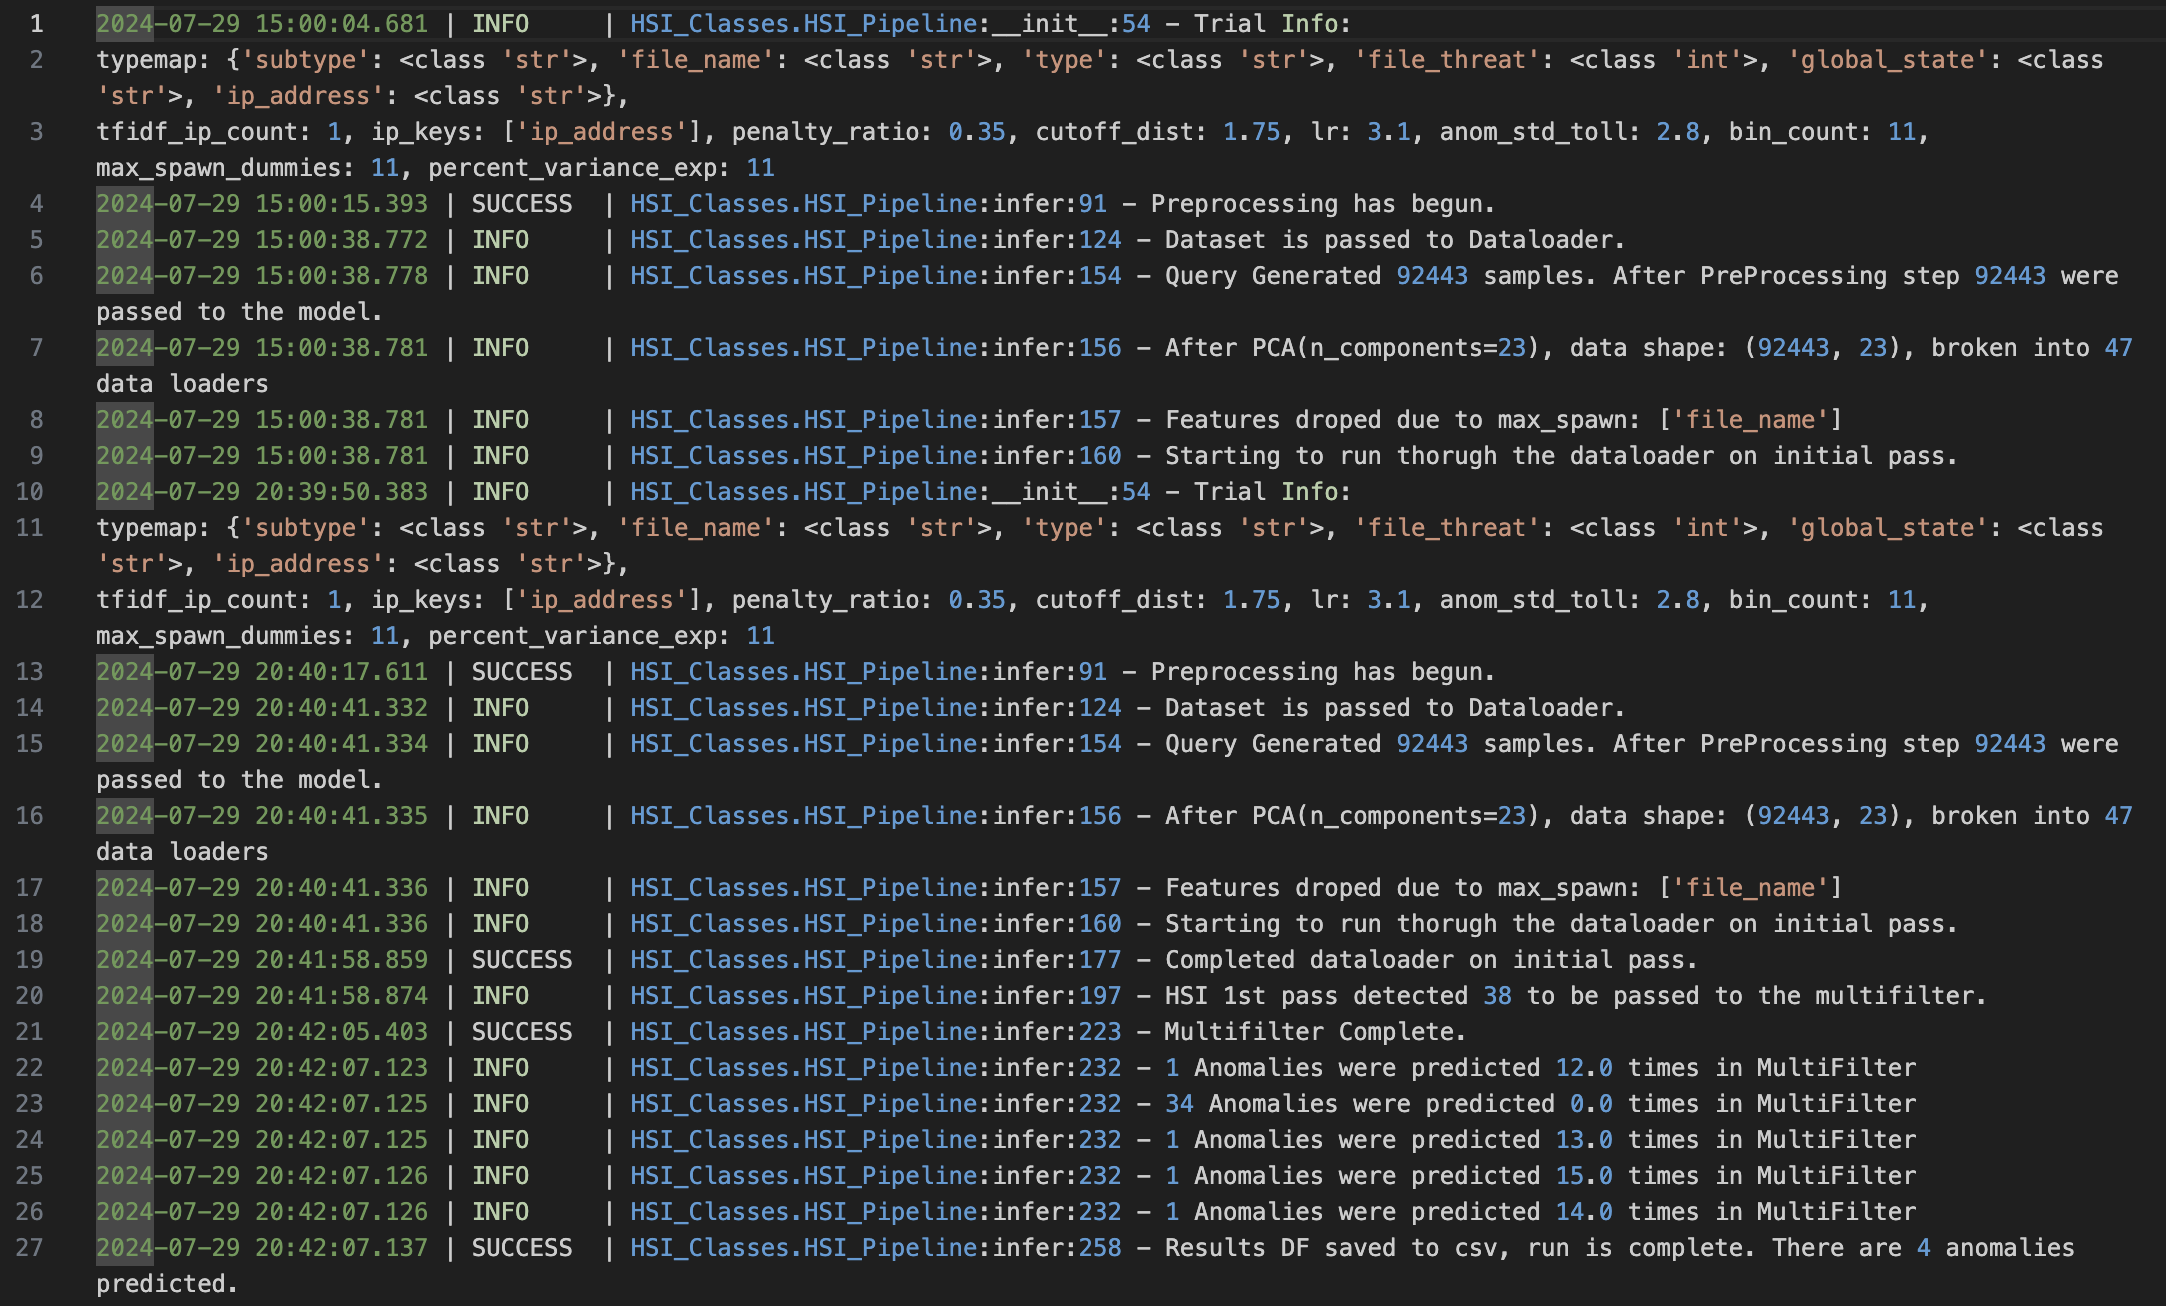
\includegraphics[clip=true, trim=.5in 0in 0in 3.3in, width=\textwidth]{../Images/Log.png}
% \end{center}


% We find:
% \begin{columns}
% \begin{column}{.5\textwidth}
% \begin{itemize}
%     \item 92,443 Events/Day
%     \item 38 Initial Predictions
% \end{itemize}
% \end{column}
% \begin{column}{.5\textwidth}
% \begin{itemize}
%     \item 34 False Positives
%     \item 4 Multifilter Anomalies  
% \end{itemize}
% \end{column}
% \end{columns}
% \end{frame}


% \begin{frame}{Example Results and Reporting}
% HSI results for this query:\\
% \begin{center}
%     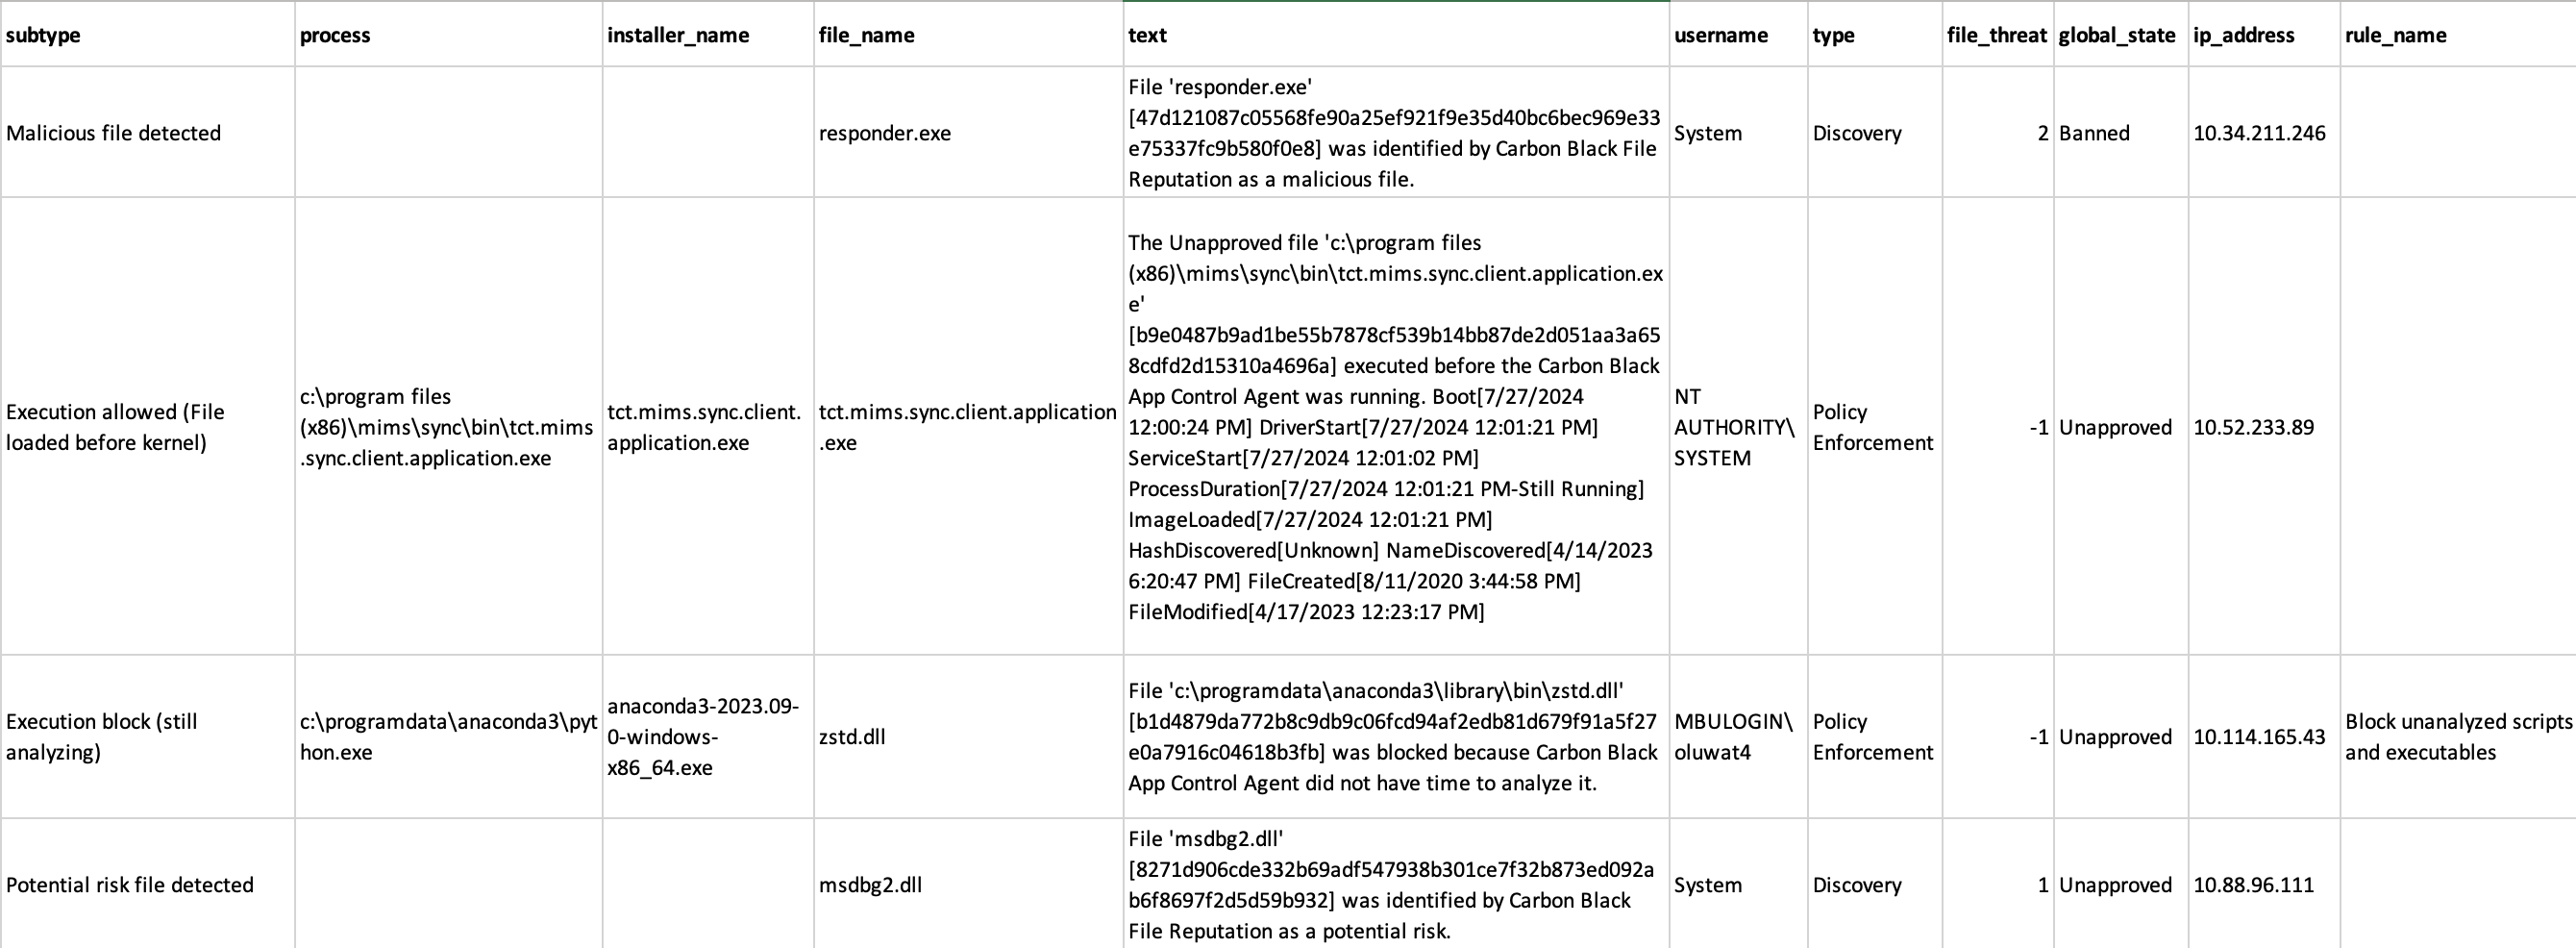
\includegraphics[ width=\textwidth]{../Images/Results.png}
% \end{center}
% \begin{itemize}
%     \item To make results actionable, \_time and IP are included in all results, regardless of their use in the model.
%     \item Results are migrated as .json to CSML1 so the universal forwarder can ingest them to ES.
% \end{itemize}

% \end{frame}
\begin{frame}{Model Structure}
    The HSI model is broken down into two main components, {weights generation} and \alert{loss function minimization}. 
    \vfill
    \bc
        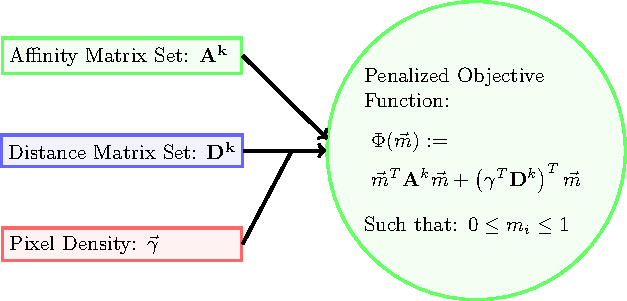
\includegraphics[width =\textwidth]{../Images/model_pipeline_tikz/Phase2_tikz/tikz.pdf}
    \ec
\end{frame}
\begin{frame}{Optimize POF$(\vec{m})$}
    Assumption: Anomalous data has a fragile relationship with background data. This relationship will not minimize the POF as well as common points. \vfill

    \textbf{HSI Pipeline:}
    \begin{itemize}
        \item A set of "evolved" matrices are kept $\vec{A}^k$
        \item Anomaly scores, $\vec{m}$, are used to minimize POF 
        \item Minimized anomaly scores are used as starting point for POF at $k+1$
        \item Once anomaly score converge with in a tolerance, optimization ends
        \item $\abs Z_{score}\abs$ is calculated for anomaly scores
    \end{itemize}\vfill
    Data points with $\abs Z_{score}\abs>$ Anomaly Threshold value are predicted. 
\end{frame}


    
\begin{frame}{Model Inference}
    % If $n$ points are passed to the model $n\times n$ comparisons are made, making the model \alert{computationally expensive}. Batching reduces statistics during model's first pass.%To reduce this demand, data is batched. This results in \alert{less data} to inform the model's statistics.
    $\mathbf{n\times n \Ria}$ Computationally Expensive / Reduced $n$ statistics
    \vfill  
    
    \textbf{Multifilter:} iterate on suspected points 
    \begin{itemize}
        \item A data frame of anomalous predictions is made from all batches predictions
        \item Upon completion of the initial pass non-anomalous data points are randomly selected from entire data set. 
        \item Anomalous data points from each batch are compared to each other, as well as, background points from the entire data set  
        \item A count of times each point is predicted anomalous is kept as a batch score 
    \end{itemize}
    \vfill
    Datapoints with batch score $<$ batch threshold are less likely to be false positives. 
\end{frame}
\begin{frame}{Model Parameter Summary}
    \vfill
Parameters that affect the HSI Model's predictions:
\vfill
    \begin{table}
        \begin{tabular}{|l|| c| r|}\hline
            \textbf{Parameter} & \textbf{Name} & \textbf{Effect}  \\\hline \hline % Is this correct?            
            $c_d$ & Cut-off Distance  &Scales $\vec{\gamma}$ and $\mathbf{A}$\\\hline
            $(P_r)^k$ & Penalty Ratio  &Decays loss contributions \\
            &$0<P_r<1$&at greater topological scales \\\hline
            $l_r$ & Learning Rate &Scales steps along\\
            & & gradient decent of POF\\\hline
            
            
            \hline\hline
            batch\_size$_d$ & Batch Size &Specifies volume of data\\
            &&available for statistics. \\\hline
            $a_t$ & Anomaly Threshold &Selects points for Multifilter\\
            &&based on $Z_{score}(\vec{m})$ \\\hline
            $m_t$ & Multifilter Threshold &Selects points for prediction\\
            &&based on multifilter count \\\hline
        \end{tabular}
    \end{table}
    \vfill
\end{frame}

\begin{frame}{Exmple Usage}
    \begin{columns}
        \begin{column}{.4\textwidth}
            Single pass of HSI:
            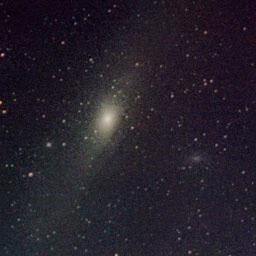
\includegraphics[width=.9\textwidth]{../Images/galaxy_256.jpeg}            
            $p\times q$ RGB channels ranging from 0-256:
            \begin{itemize}
                \item Ravel to $(p\times q, 3)$
                \item Scale
                \item HSI Inferences
                \item Heat map $\vec{m}$  as $p\times q$
            \end{itemize}
        \end{column}
        \begin{column}{.67\textwidth}
            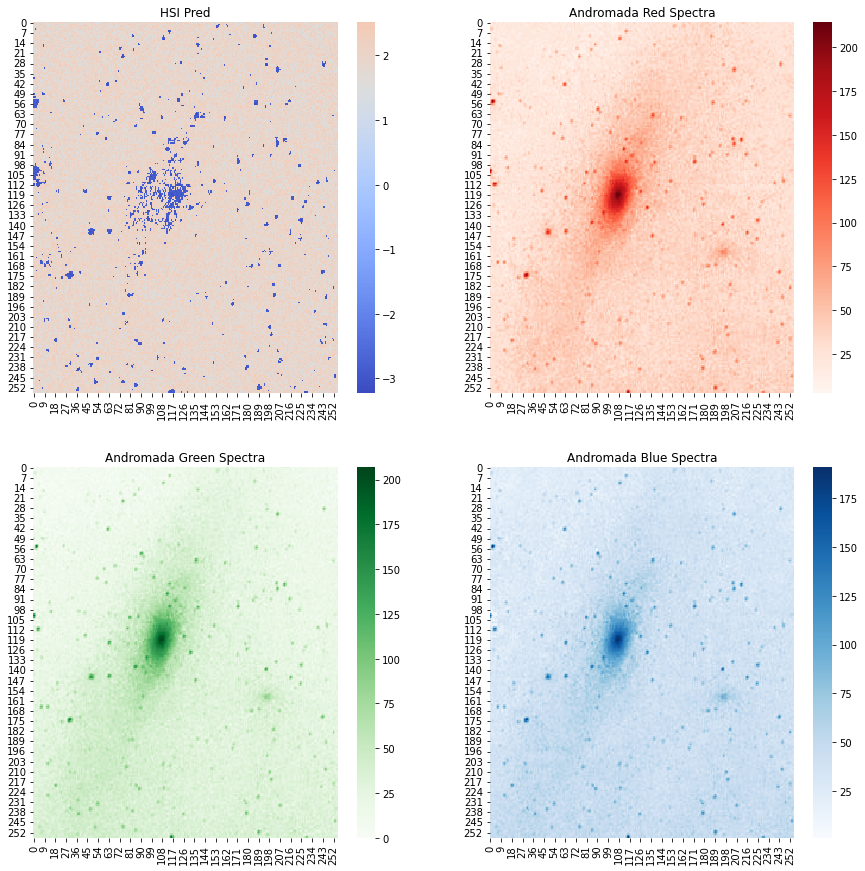
\includegraphics[width=\textwidth]{../Images/MicrosoftTeams-image.png}            
        \end{column}
    \end{columns}
\end{frame}
\begin{frame}{Exmple Usage}
    \begin{columns}
        \begin{column}{.66\textwidth}
            Single pass of HSI:       
            $p\times q$ Internet Protocol Data:
            \begin{itemize}
                \item Time series parsing of the Carbon-Black Logs
                \item Preprocessing: Encoding, Scaling, and PCA
                \item HSI Inferences
                \item Multi-filtered
                \item Multi Filter Count
            \end{itemize}
        \end{column}
        \begin{column}{.33\textwidth}
            \bc
            \vspace{-.5in}
            \begin{figure}               
                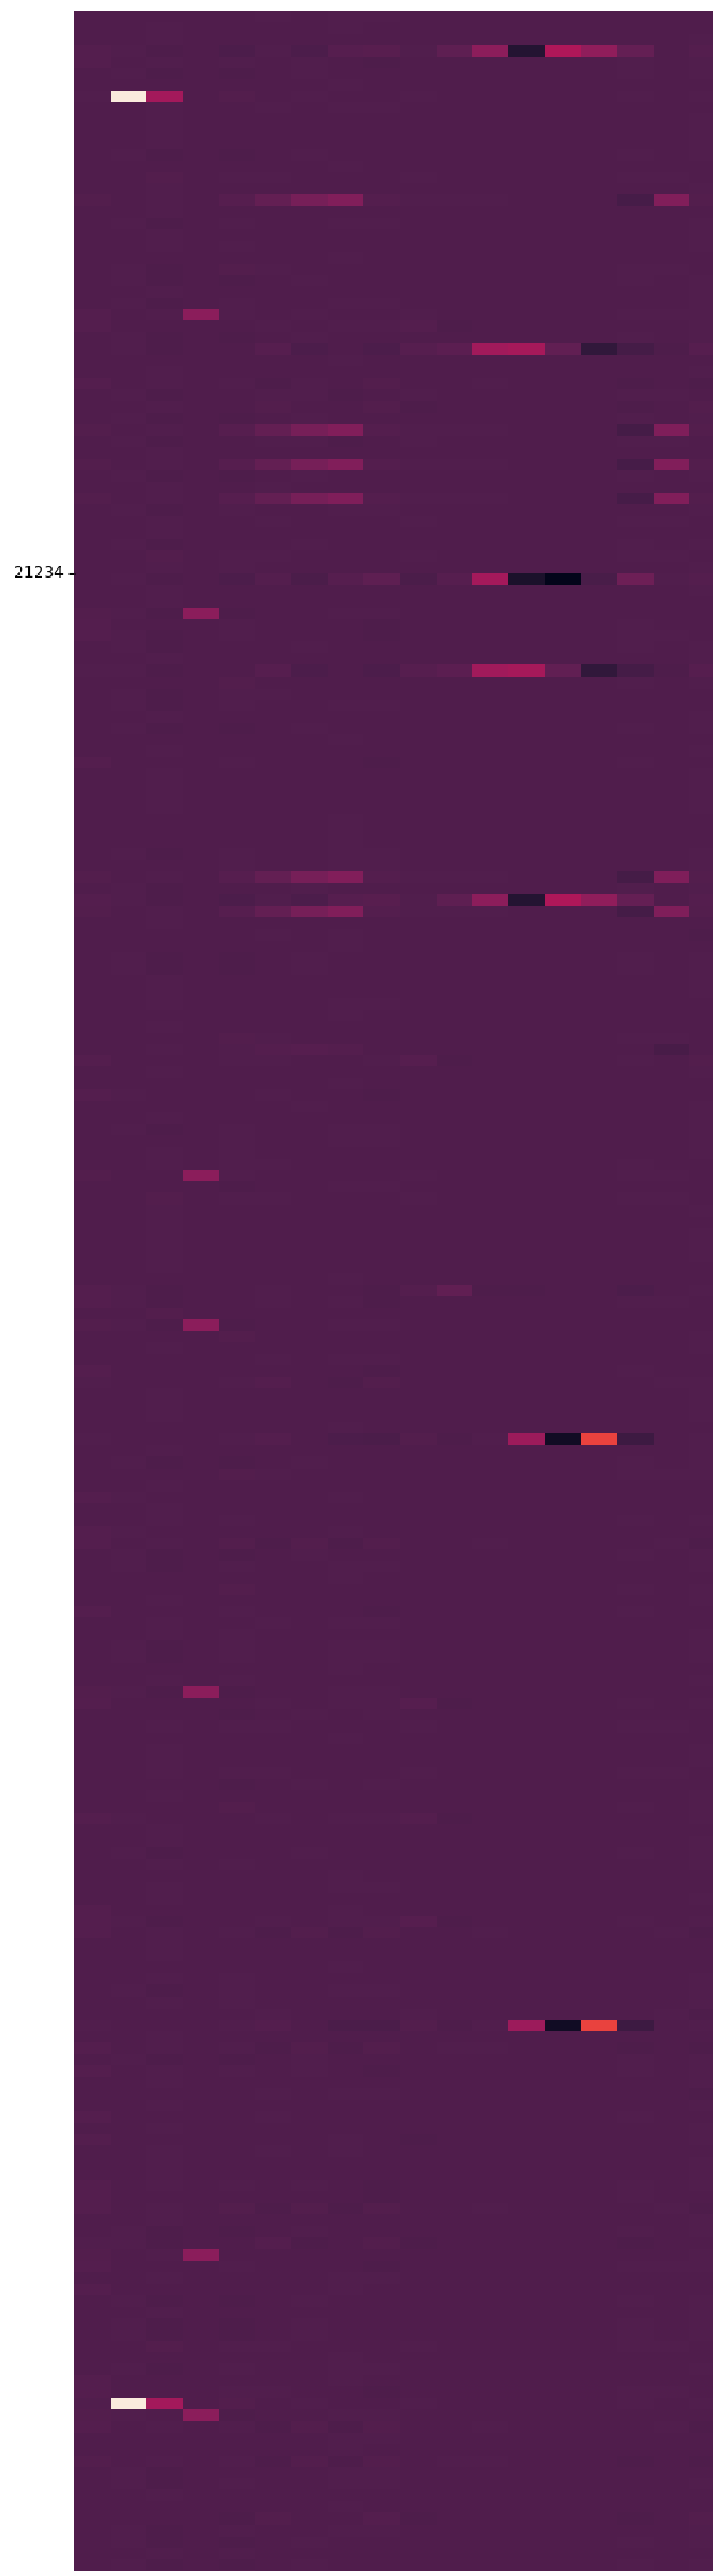
\includegraphics[height=.7\textheight]{../Images/model_pipeline_tikz/CyberPred/raw_data.pdf} 
            \caption{Preprocessed input data relevant to Cyber Security.}       
            \end{figure}
            \ec
        \end{column}
    \end{columns}
\end{frame}


\begin{frame}{Exmple Usage}
    \begin{columns}
        \begin{column}{.66\textwidth}
            Single pass of HSI:       
            $p\times q$ Internet Protocol Data:
            \begin{itemize}
                \item Time series parsing of the Carbon-Black Logs
                \item Preprocessing: Encoding, Scaling, and PCA
                \item HSI Inferences
                \item Multi-filtered
                \item Multi Filter Count
            \end{itemize}
        \end{column}
        \begin{column}{.33\textwidth}
            \bc
            \vspace{-.5in}
            \begin{figure}               
                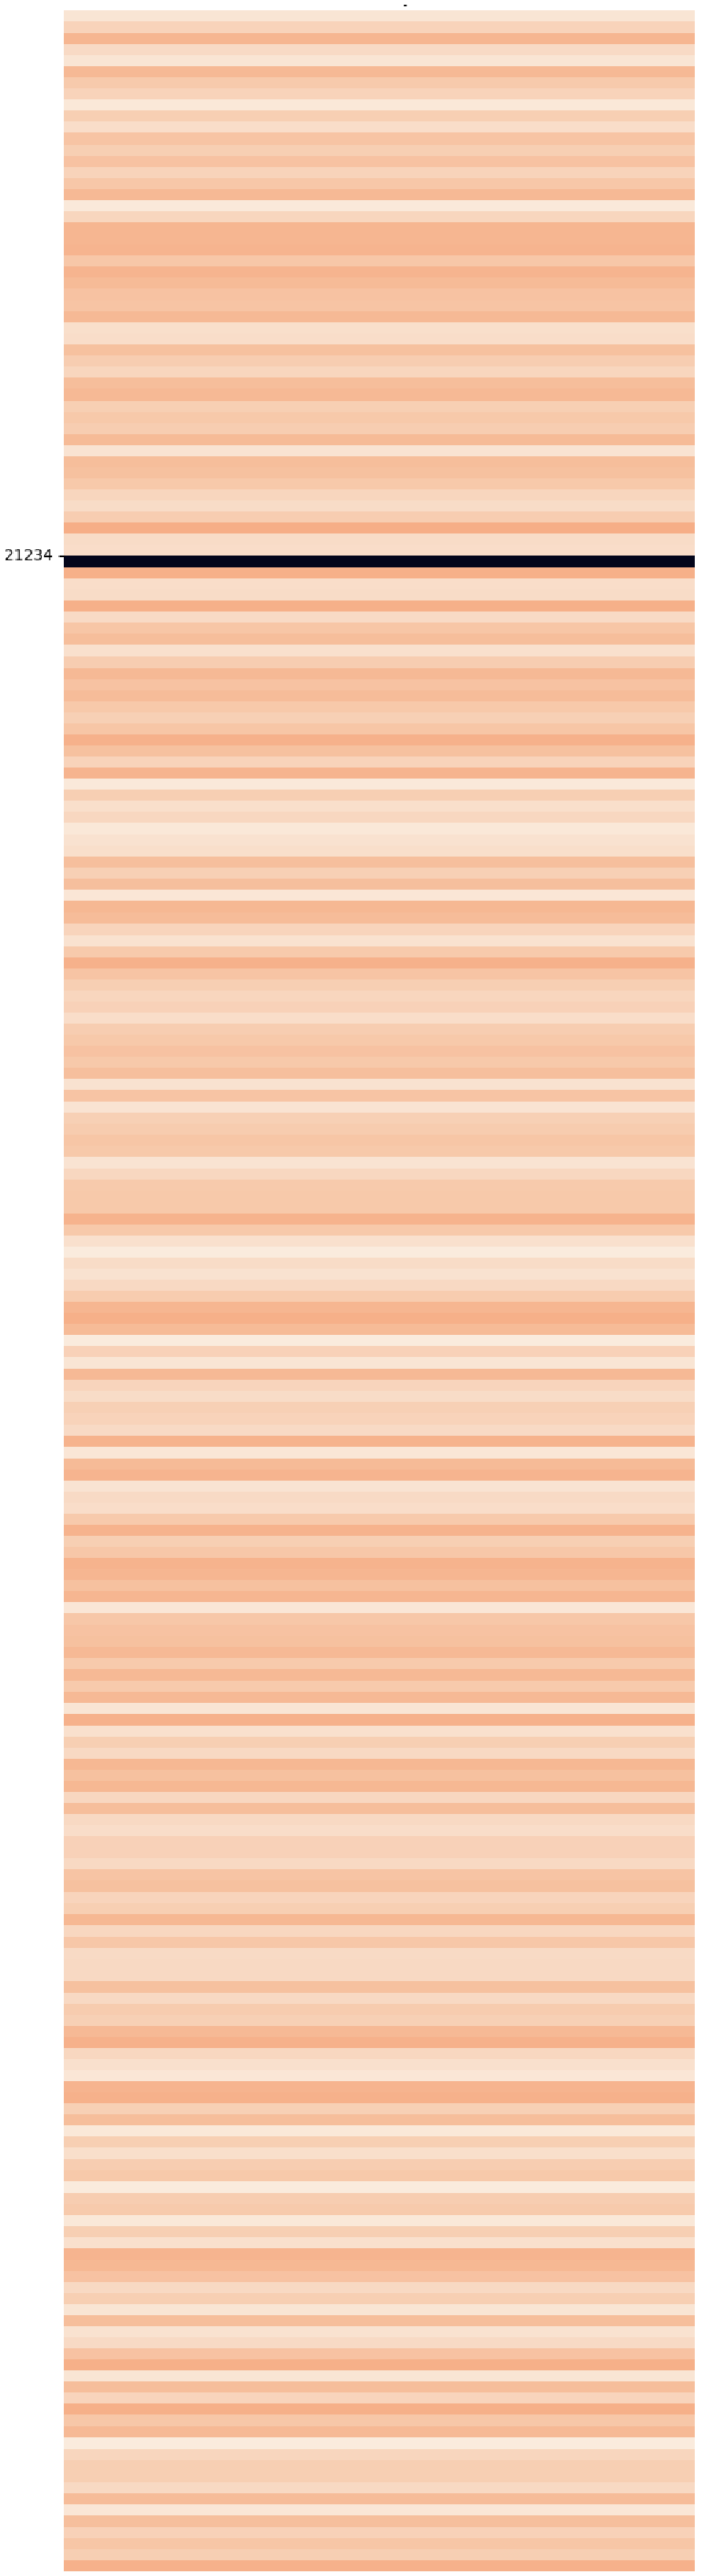
\includegraphics[height=.7\textheight]{../Images/model_pipeline_tikz/CyberPred/anomaly_score.pdf} 
            \caption{Multi-filter count after 15 filters. Max value of 13. }       
            \end{figure}
            \ec
        \end{column}
    \end{columns}
\end{frame}


\begin{frame}{Exmple Usage}
    \begin{columns}
        \begin{column}{.66\textwidth}
            Multi-filtered HSI:       
            $p\times q$ Internet Protocol Data:
            \begin{itemize}
                \item Time series parsing of the Carbon-Black Logs
                \item Preprocessing: Encoding, Scaling, and PCA
                \item HSI Inferences
                \item Multi-filtered
                \item Multi Filter Count
            \end{itemize}
        \end{column}
        \begin{column}{.33\textwidth}
            \bc
            \vspace{-.5in}
            \begin{figure}               
                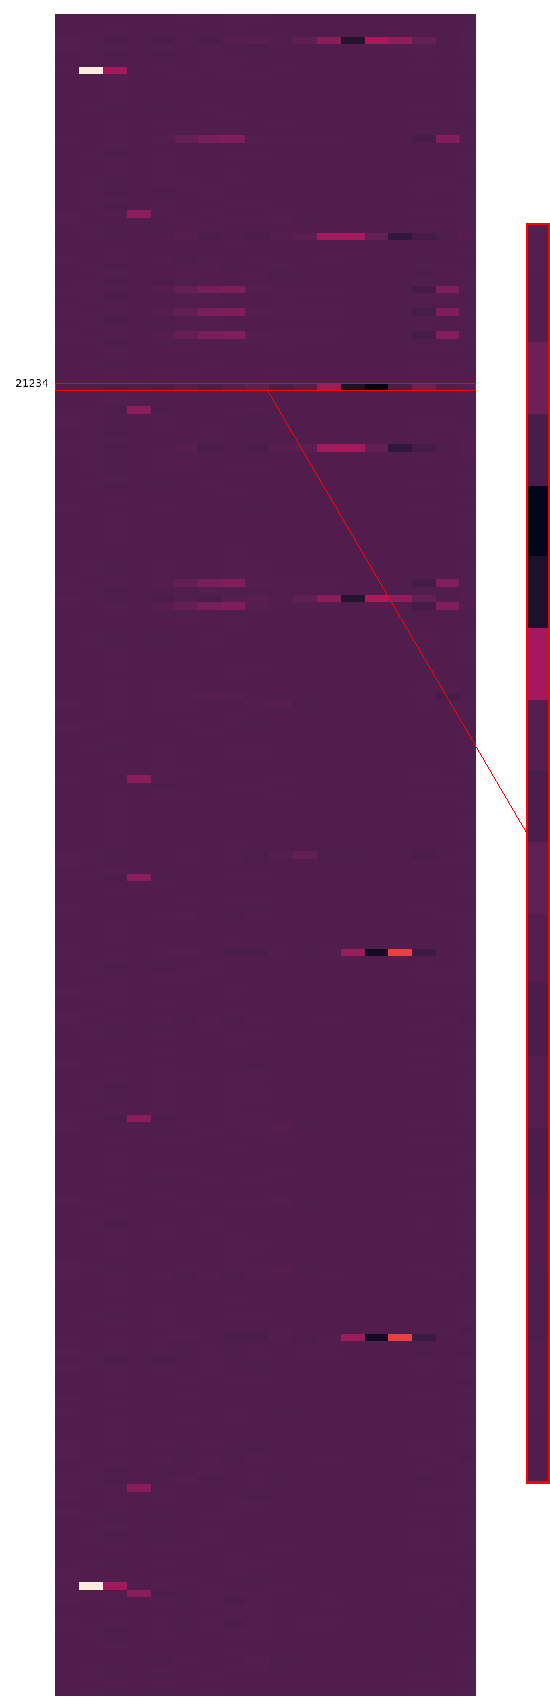
\includegraphics[height=.7\textheight]{../Images/model_pipeline_tikz/CyberPred/anomaly_raw_data.pdf} 
            \caption{Anomalous data point predicted by the HSI model. }       
            \end{figure}
            \ec
        \end{column}
    \end{columns}
\end{frame}

\begin{frame}{Closing}
    \textbf{Observations:}
    \begin{itemize}
        \item Generalizable to data types
        \item Effective in Cyber Tasks
        \item Computation time scales batch\_size$^2$
    \end{itemize}
    \vfill
    \textbf{Future Work:}
    \begin{itemize}
        \item Test model on new data sources\dots Audio, .etc
    \end{itemize}
    \vfill
    \textbf{Conclusion:}\\
    The HSI model has been implemented on image and cyber security related data. The model has been used to identify actionable malicious behaviors in IP data.
    \vfill
    \bc
    \textbf{Questions?}
    \ec
    \vfill


\end{frame}
\usebackgroundtemplate{
\includegraphics[width=\paperwidth,page=3]{../Images/Presentation1.pdf}}%
\begin{frame}{}
\end{frame}
% This document must be compiled from the main.tex all others will cause a compile error
% Beamer takes forever to compile, so I use this format to work on 1 slide at a time.  When all slides are complete do one compile with all slides or sections included.

\end{document}